\subsection{Classifieurs par profils et histogrammes horizontaux et verticaux}
\subsubsection{Présentation de la méthode}
Le premier classifieur développé se base sur la détermination de vecteurs caractéristiques de la main à reconnaitre. Il a été subdivisé en deux sous classes, dont chacune se base sur une caractéristique différente. Ce classifieur travaille sur les images des mains segmentées et extraites de l'image originale.

La première classe s'intéresse aux profils de la main à détecter, soit la distance entre les bordures gauches et droites, hautes et basses, et le premier pixel constituant la main à traiter, et ce pour un certain nombre de lignes régulièrement espacées. Sur le même principe, les profils verticaux sont générés.

\begin{figure}[htb!]
\centerline{
\includegraphics{profilsVert.png}}
\caption{Profils verticaux d'une main.}
\end{figure}

\begin{figure}[htb!]
\centerline{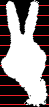
\includegraphics{profilsHoriz.png}}
\caption{Profils horizontaux d'une main.}
\end{figure}

Ainsi, on détermine la morphologie globale de la main à traiter. Il est à noter que tous les profils sont normalisés (par division par la largeur en pixel de chaque image traitée), et ce afin de pouvoir être comparés entre eux, chaque main traitée ayant des dimensions différentes.

La seconde classe quant à elle s'intéresse aux histogrammes. Pour un certain nombre de lignes, on compte le nombre de pixels constitutifs de la main à traiter (dans notre cas, les pixels blancs), afin de déterminer non pas la morphologie de la main à reconnaitre, mais la densité de la ligne considérée. Selon le même principe, l'histogramme d'un certain nombre de colonnes est calculé. Ces histogrammes sont également normalisés afin de pouvoir comparer des images de dimensions différentes.

Le nombre de lignes à considérer est paramétrable à travers la variable NB\_PROFILES. Cette variable représente en effet le nombre de lignes et de colonnes à considérer pour déterminer les profils ou les histogrammes horizontaux et verticaux. Plus le nombre de lignes considérées est important, plus le profil global du caractère sera précis. Par conséquent, ce paramètre a une influence directe très importante sur le taux de reconnaissance des mains, mais également sur le coût d’exécution. Si une valeur trop basse est choisie, la détection de la morphologie de la main risque d’être trop peu significative pour obtenir des résultats probants. A l’inverse si une valeur trop élevée est choisie, la différence entre deux mains d’une même classe sera évaluée comme étant importante. Par ailleurs, l'augmentation du nombre de lignes à évaluer induit également une augmentation du temps de traitement des images.

	Afin de disposer de points de comparaisons pour l'image à traiter, on établit une base de référence, subdivisée en un certain nombre de classes représentant chacune un nombre de doigts. Basiquement, la base est constituée de 6 classes, numérotées de 0 à 5 et constituées chacune d'un certain nombre d'images de références présentant le nombre de doigts correspondant à la classe en question. Pour établir cette base, on traite toutes les images de chaque classe afin de déterminer les vecteurs caractéristiques, profils ou histogrammes. Une fois toutes les images de la base traitées, on établit une moyenne des profils ou des histogrammes de chaque classe, afin d'obtenir le vecteur caractéristique de chaque classe de la base. C'est à partir de ces vecteurs moyens que chaque image à reconnaitre sera comparée. 	

	La comparaison s'effectue par distance euclidienne entre le vecteur caractéristique moyen de chaque classe et le vecteur caractéristique de l'image à reconnaitre. Les vecteurs caractéristiques horizontaux et verticaux sont combinés en un seul par simple concaténation. On obtient ainsi la distance de l'image traitée à chacune des classes. Plus cette distance est faible, plus l'image à reconnaitre présente de similarités avec la classe en question. Ces distances à chaque classe sont par ailleurs transformées en taux de probabilité, à travers la formule :

\[
P(\omega_i / x) = \frac{exp(-d(x, \omega_i))}{\sum_{j=0}^{k}-d(x, \omega_j)}
\]

où $\omega_i$ est la classe $i$, $x$ est l'image traitée et $d$ est la distance euclidienne.

Il est à noter que les 6 classes de la base, représentant le nombre de doigts, peuvent être subdivisées en sous classes. En effet, pour un même nombre de doigts, une main peut présenter des configurations différentes. Par exemple, pour présenter deux doigts, il est fréquent de rencontrer deux configurations de la main : la première présentant le pouce et l'index, la seconde présentant l'index et le majeur. Hors, ces deux configurations différentes pour un même nombre de doigt présentent des vecteurs caractéristiques très différent l'un de l'autre. C'est la raison pour laquelle il est possible de distinguer ces configurations de la main au sein de différentes classes, auxquelles on associe le nombre de doigts correspondant.

	Par ailleurs, une seconde méthode de prise de décision a été implémentée, celle des K plus proches voisins. Pour ce faire, le vecteur caractéristique de l'image à traiter est comparé non plus avec le vecteur caractéristique moyen de chaque classe, mais avec ceux de l'intégralité des images constitutives de la base d'apprentissage. On retient ainsi les K images les plus proches, puis nous calculons les probabilités d'appartenance aux classes de la main à traiter par représentation de chaque classe parmi les K plus proches.

\subsubsection{Résultats}

Les résultats obtenus sont très aléatoires, en fonction des différents paramètres intervenant. Ainsi, d'une base d'apprentissage à une autre, d'une image testée à une autre, le taux de réussite oscille entre 20\% et plus de 80\%, en atteignant parfois 100\% pour certaines séries d'images. Cependant les résultats restent très irréguliers, et restent en moyennent autours de 50\% de réussite. Par ailleurs, une combinaison de ces deux classifieurs donne également des résultats très irréguliers, parfois améliorant quelque peut le taux de détection, parfois le dégradant. Nous pensons que la base d'apprentissage constituée reste trop restreinte pour permettre d'obtenir des résultats probants. 

Dans tous les résultats suivant, voici la correspondance des différents paramètres :
\begin{itemize}
\item Base d'apprentissage 1 : une base d'apprentissage simple, composée de 6 classes, et  constituée d'images présentant une configuration assez simple.
\item Base d'apprentissage 2 : une base d'apprentissage étendue, composée de 12 classes en différenciant certaines configuration de la main pour un même nombre de doigts.
\item Série 1 : les images de la base d'apprentissage 1.
\item Série 2 : les images de la base d'apprentissage 2.
\item Le paramètre "redressées" indique si les images ont subit un redressement ou non.
\end{itemize}

Voici une série de résultats des classifieurs par profils et par histogramme, en fonction de la base d'apprentissage, de la série d'images testée, et du nombre de lignes considérées: (\autoref{fig:resultatsClass1}).

\begin{figure}[htb!]
\centerline{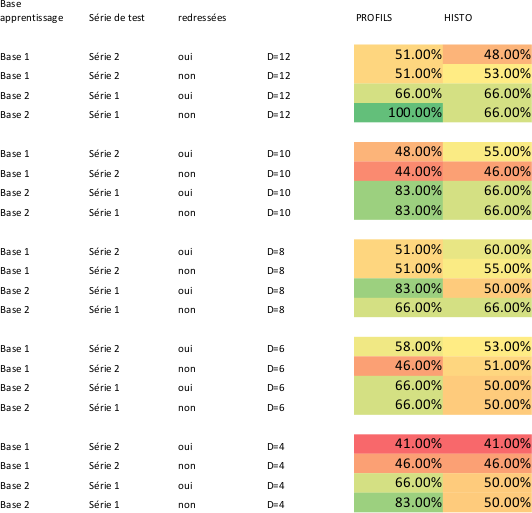
\includegraphics[scale=0.7]{table.png}}
\caption{Résultats du classifieur profils et histogrammes verticaux/horizontaux avec distance Euclidienne.}
\label{fig:resultatsClass1}
\end{figure}

Considérant que le meilleur compromis est atteint pour D = 8, voici une seconde série de résultats obtenus par la méthode des KPPV, K variant de 3 à 6 : (\autoref{fig:resultatsKPPV}).

\begin{figure}[htb!]
\centerline{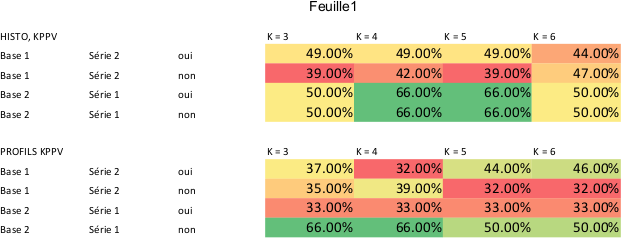
\includegraphics[scale=0.7]{table1.png}}
\caption{Résultats du classifieur profils et histogrammes verticaux/horizontaux avec KPPV.}
\label{fig:resultatsKPPV}
\end{figure}

\subsubsection{Améliorations possibles}
L'amélioration la plus importante à apporter est probablement l'enrichissement de la base d'apprentissage. En effet, nos bases actuelles disposent de trop peu d'images, ce qui génère des différences importantes entre les images de la base et certaines configurations hasardeuses de la main à tester.

	Une seconde amélioration envisagée serait de pondérer la prise en compte des caractéristiques des différentes zones de l'image à tester, notamment en augmentant le poids des mesures effectuées sur la partie supérieure de la main, là où se trouvent les doigts. A l'inverse, il serait intéressant de réduire l'importance des mesures effectuées dans la partie basse de l'image, zone dans laquelle se trouve le poignet que la segmentation ne permet pas toujours d'éliminer. Cependant, il faudrait pour ce faire disposer d'une fonction de redressement des mains moins hasardeuse. En effet, certaines images sont tout bonnement redressées à l'envers, ce qui fausse la comparaison par la suite.

	Enfin, la méthode de décision basée sur les KPPV peut également être améliorée. Dans le cas où plusieurs classes seraient équi-représentées, la classe actuellement retournée est la première ayant atteint la représentation maximale. Il serait judicieux de retourner la classe représentée dont la distance à une image de la base est la plus faible.

\subsection{Classifieur densités}

Le second classifieur implémenté s'intéresse à la densité de l'image à traiter. Chaque image (après segmentation et extraction de la main) est subdivisée en plusieurs zones de tailles égales. Puis, pour chaque zone, on détermine le nombre de pixels appartenant à la main (dans notre cas les pixels blanc). Ce nombre de pixel est ensuite normalisé, par division par le nombre total de pixel de la zone. On obtient ainsi la densité des différentes zones de l'image.

	Sur le même principe que pour les classifieurs précédents, on établit une base d'apprentissage divisée en plusieurs classes correspondant au nombre de doigts. Chaque classe de la base est constituée d'un certain nombre d'images présentant des mains du nombre de doigts correspondant à la classe. Chaque image à traiter est comparée avec cette base, et l'on obtient un vecteur de probabilité de chaque classe sur le même modèle que précédemment.

	Par ailleurs, le nombre de subdivisions de l'image est également paramétrable via les variables M et N. A nouveau, ce nombre de zones a une influence importante sur le taux de détection. Un nombre trop faible ne permettra pas d'obtenir une carte de densité suffisamment précise pour obtenir des résultats satisfaisants. A l'inverse, un trop grand nombre de zones peut produire des écarts importants, et le taux de reconnaissance se dégrade.

\subsubsection{Résultats}
\begin{figure}[htb!]
\centerline{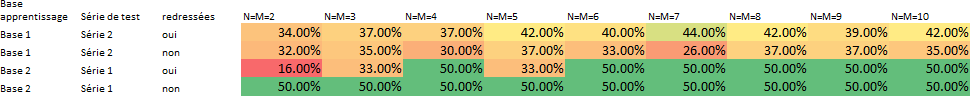
\includegraphics[scale=0.7]{table2.png}}
\caption{Résultats du classifieur densités avec distance euclidienne.}
\end{figure}

\begin{figure}[htb!]
\centerline{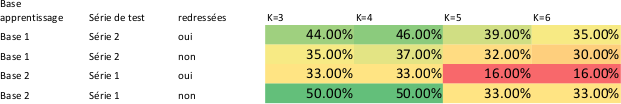
\includegraphics[scale=0.7]{table3.png}}
\caption{Résultats du classifieur densités avec KPPV.}
\end{figure}